\documentclass[a4paper,12pt]{article}
%\usepackage[utf8x]{inputenc}
\usepackage{amssymb}
\usepackage{amsfonts}
\usepackage{mathrsfs}
\usepackage{amsmath}
\usepackage{amsthm}
\usepackage[margin=3cm]{geometry}
\usepackage{times}
\usepackage{graphicx}
%\usepackage{enumitem}
\usepackage{fancyhdr}
\usepackage{hyperref}
\usepackage{setspace}
\usepackage{subcaption}
\usepackage{mathtools}
\usepackage{siunitx}

\pagestyle{fancy}
\fancyhf{}
\lhead{Thomas J. Delaney}
\rhead{Recurrent neural network implementations}
\cfoot{\thepage}

\newtheorem{theorem}{Theorem}
\newtheorem{proposition}{Proposition}[section]
\newtheorem{lemma}{Lemma}[section]
\newtheorem{corollary}{Corollary}[section]
\theoremstyle{definition}
\newtheorem{definition}{Definition}[section]

\newcommand{\boldnabla}{\mbox{\boldmath$\nabla$}} % to be used in mathmode
\newcommand{\cbar}{\overline{\mathbb{C}}}% to be used in mathmode
\newcommand{\diff}[2]{\frac{d #1}{d #2}}% to be used in mathmode
\newcommand{\difff}[2]{\frac{d^2 #1}{d #2^2}}% to be used in mathmode
\newcommand{\pdiff}[2]{\frac{\partial #1}{\partial #2}} % to be used in mathmode
\newcommand{\pdifff}[2]{\frac{\partial^2 #1}{\partial #2^2}}% to be used in mathmode
\newcommand{\upperth}{$^{\mbox{\footnotesize{th}}}$}%to be used in text mode
\newcommand{\vect}[1]{\mathbf{#1}}% to be used in mathmode
\newcommand{\curl}[1]{\boldnabla \times \vect{#1}} % to be used in mathmode
\newcommand{\divr}[1]{\boldnabla \cdot \vect{#1}} %to be used in mathmode
\newcommand{\modu}[1]{\left| #1 \right|} %to be used in mathmode
\newcommand{\brak}[1]{\left( #1 \right)} % to be used in mathmode
\newcommand{\comm}[2]{\left[ #1 , #2 \right]} %to be used in mathmode
\newcommand{\dop}{\vect{d}} %to be used in mathmode
\newcommand{\cov}{\text{cov}} %to be used in mathmode
\newcommand{\var}{\text{var}} %to be used in mathmode
\newcommand{\mb}{\mathbf} %to be used in mathmode
\newcommand{\bs}{\boldsymbol} %to be used in mathmode
% Title Page
\title{Recurrent neural network implementations on the M4 dataset}
\date{}
\author{Thomas J. Delaney}

\begin{document}

\maketitle

\tableofcontents

\newpage

\section{Introduction}
The purpose of this document is to describe the recurrent neural networks (RNNs) applied to the M4 dataset as an attempt to forecast the financial series in the M4 dataset.

\section{Objectives}
Our main objective in this experiment was to create a forecasting method similar to that of Smyl et al (2018), which won the M4 forecasting competition \cite{smyl}. More specifically, we wanted to create forecasting method that blended statistical forecasting with machine learning methods using recurrent neural networks. So, our aims were:
\begin{itemize}
  \item To train non-seasonal and seasonal forecasting methods using statistical techniques and RNNs together.
  \item To use these methods to forecast the financial series in the M4 dataset.
  \item To compare the performance of these methods to simpler statistical methods.
  \item To compare the performance of these methods to the M4 winning statistical-RNN hybrid model.
\end{itemize}
Our hope (rather than expectation) was that a model simpler than that in \cite{smyl} could be used to forecast the financial time series.

\section{Background}
For background on the M4 competition, see \cite{m4} or \cite{meta}.

The winner of the M4 competition was a hybrid forecasting model that combined simple exponential smoothing methods with recurrent neural networks. It was developed by Slawek Smyl while working at Uber. In this model, simple exponential smoothing is used to estimate a multiplicative level and seasonality of each time series. These level and seasonality components are used to scale the time series before the time series is passed to the RNN. An RNN with a different architecture is used for each time series frequency. Each RNN uses LSTM cells and dilation, and the  attention mechanism is used for some frequencies. 

The learning mechanism and model is hierarchical in nature. The exponential smoothing parameters are learned for each individual time series, whereas the weights in the RNN are learned across all the scaled time series. For more information on this model see \cite{smyl} or \cite{lit}. For more information on recurrent neural networks, see \cite{lit}.

The statistical modelling in this experiment was performed in \texttt{R} using the \texttt{forecasting} package. We specifically used an \textit{ets model} for modelling both seasonal and non-seasonal data. For more information about ets models, other statistical models, and the \texttt{forecasting} package see \cite{fpp}. 

The RNNs in this experiment we created and trained in \texttt{R} using \textit{RStudio} and \textit{Keras}. Keras is a high-level neural networks API enabling quick and easy building of and experimentation with neural networks. We used \textit{tensorflow} as the back-end for Keras. For for information on Keras, see \cite{keras}. For more information on Tensorflow, see\cite{tf}.

\section{Methods}

\subsection{Statistical Modelling}\label{sec:stats_modelling}
In this section, we describe the statistical models applied to the time series. Bare in mind that these models were not intended to accurately model or forecast the time series. The intention was to use the level and seasonal components extracted to scale the time series before passing the scaled series into the RNN.

\subsubsection{Non-seasonal}\label{sec:non_seasonal_stats_modelling}
To statistically model the yearly time series, we used a non-seasonal ETS model with a multiplicative error and no trend component. This models the time series as a level component with multiplicative white noise error. The model is defined by
\begin{align}
	y_t &= \ell_{t-1}(1 + \epsilon_t) \label{eq:non_seasonal_series} \\
	\ell_t &= \ell_{t-1}(1 + \alpha \epsilon_t) \label{eq:non_seasonal_level}
\end{align}
where $y_t$ is the time series, $\ell_t$ is the level component, and $\alpha$ is a smoothing parameter.

\subsubsection{Seasonal}\label{sec:seasonal_stats_modelling}
To statistically model quarterly time series, we used an ETS model with a multiplicative seasonality, multiplicative error, and no trend component. This models the time series as a level component with a multiplicative seasonal component, and a multiplicative white noise error. The model is defined by
\begin{align}
	y_t &= \ell_{t-1}s_{t-m}(1 + \epsilon_t) \label{eq:seasonal_series} \\
	\ell_t &= \ell_{t-1}(1 + \alpha \epsilon_t) \label{eq:seasonal_level} \\
	s_t &= s_{t-m}(1 + \gamma \epsilon_t) \label{eq:seasonal_season}
\end{align}
where $y_t$ is the time series, $\ell_t$ is the level component, $\alpha$ is a level smoothing parameter, $s_t$ is the seasonal component, $\gamma$ is the seasonal smoothing parameter, and $m$ is the number of time points (or seasons) in a full seasonal cycle (e.g. $4$ for quarterly data).

\subsection{Recurrent Neural Network}
The RNN that we used in this experiment is fairly simple compared to those used in \cite{smyl}. Time constraints were the main reason for this. The network consisted of an input layer, two hidden layers, and an output layer. 

The first hidden layer consisted of $32$ gated recurrent units (GRUs), with $\tanh$ output activation and \textit{hard sigmoid} recurrent activation (see \ref{sec:hard_sigmoid}). A standard dropout rate of $10\%$ and recurrent dropout rate of $50\%$ were implemented.

The second hidden layer consisted of $64$ GRUs. This time a rectified linear unit output activation was used.The same dropout rates were used.

The output layer consisted of a number of densely connected units equal to the number of points to be forecast ($6$ for yearly, $8$ for quarterly).

Note that we used only the last $30$ elements of each time series in our model. This was to keep the training time reasonable short. We also felt that given the forecast horizon for the non-seasonal data was $6$ time steps, and the forecast horizon for seasonal data was $8$ time steps, $30$ time steps should be enough to train a model for forecasting. 

\subsubsection{Hard sigmoid activation function}\label{sec:hard_sigmoid}
The hard sigmoid function is a piece-wise linear approximation of the sigmoid function. When plotted in two dimensions, the function consists of three linear segments, one along the x-axis, one with a slope of $\frac{1}{5}$ and intercept of $\frac{1}{2}$, and one parallel to the x-axis with $f(x) = 1$. The function can be defined by 
\begin{align}
	f(x) = \begin{cases}
		0, &\text{ if } x < -\frac{5}{2} \\
		\frac{x}{5} + \frac{1}{2}, &\text{ if }  -\frac{5}{2} \leq x \leq \frac{5}{2} \\
		1, &\text{ if } x > \frac{5}{2}
	\end{cases}
\end{align}
Figure \ref{fig:sigmoid} shows the standard sigmoid and the hard sigmoid over the domain $[-10, 10]$ for comparison \footnote{See the code of the keras implementation of this function in Python here: \url{https://github.com/keras-team/keras/blob/master/keras/backend/tensorflow\_backend.py\#L3394}}.

\begin{figure}[ht]
	\centering
	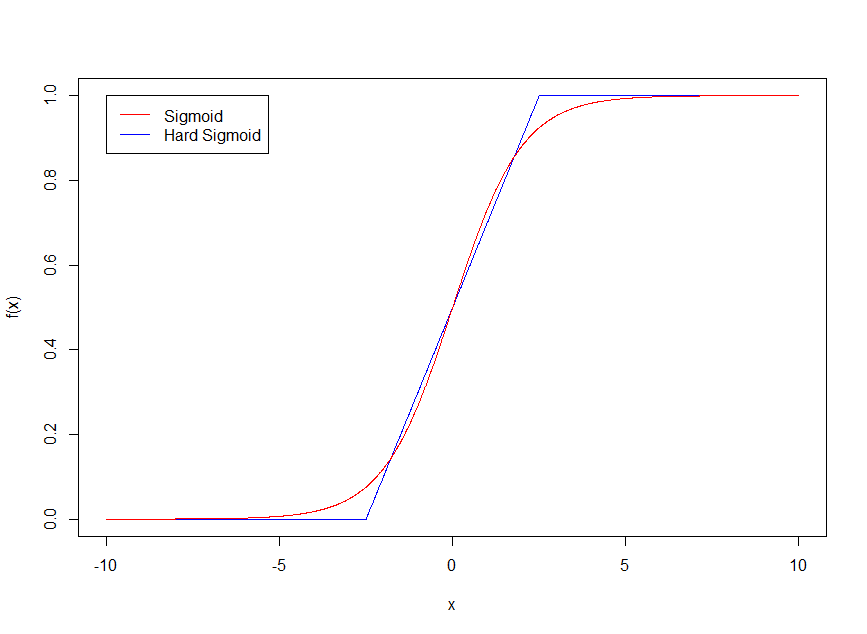
\includegraphics[width=\textwidth]{figures/sigmoid.png}
	\caption{The sigmoid and hard sigmoid functions. The hard sigmoid is a linear approximation of the sigmoid that is commonly used as the recurrent activation in GRU or LSTM networks.}
	\label{fig:sigmoid}
\end{figure}

This function is commonly used in place of the sigmoid function because it's much quicker to calculate the hard sigmoid. Specifically, the calculations for $e^{-x}$ are no longer necessary, and only linear operations need to be performed. 

\subsection{Combining the statistical model and RNN}
\subsubsection{Non-seasonal}
In order to combine the statistical model with the recurrent neural network, and attempt to use the power of both we did the following:
\begin{enumerate}
	\item We split the dataset of non-seasonal M4 series into training, validation, and test sets.
	\item We fit the non-seasonal ETS model described in section \ref{sec:non_seasonal_stats_modelling} to each of the training series. This returned a level series, and a residual series for each time step in each series. 
	\item We trained the RNN to forecast the residual series, using the mean absolute error as the loss function. If we examine equation \ref{eq:non_seasonal_series}, we can see that forecasting the residuals is equivalent to forecasting a scaled and translated version of the time series, namely $\frac{y_t}{\ell_{t-1}} - 1$.
	\item In order to obtain a descaled and detranslated forecast, we used the values for $\epsilon_t$ given to us by the RNN output along with equations \ref{eq:non_seasonal_series} and \ref{eq:non_seasonal_level} to calculate $y_t$ and $\ell_t$ for each timestep in the forecast horizon.
\end{enumerate}

We used the validation set during the training of the RNN, and to quantify the performance of our hybrid method compared to the baseline method.

\subsubsection{Seasonal}
The process for the seasonal time series was similar to that for the non-seasonal, except that the fitted ets model (as described in section \ref{sec:seasonal_stats_modelling}) returned a seasonal series as well as a level series and a residual series. The residual series was equivalent to $\frac{y_t}{\ell_{t-1}s_{t-1}} - 1$ In order to obtain the final forecast, we had to use the level and seasonal series with equations \ref{eq:seasonal_series}, \ref{eq:seasonal_level}, and \ref{eq:seasonal_season} to descale and deseasonalise the output of the RNN.

\subsection{Baseline Methods}
In order to assess the performance of our hybrid model, we compared its forecasting performance to that of a simpler statistical model. We chose different simple models for non-seasonal and seasonal data.

\subsubsection{Non-seasonal}\label{sec:baseline_methods_non_seasonal}
For non-seasonal forecasting we used a random walk model with a drift component as the baseline model.

\subsubsection{Seasonal}\label{sec:baseline_methods_seasonal}
For seasonal forecasting, we used a seasonal na{\"i}ve method as the baseline model.

%\subsection{Meta-learning method comparison}
%The forecasting method that finished second in the M4 competition was a \textit{meta-learning method} in which the optimal weightings for a weighted average of various statistical methods was learned. For more information on this method, see \cite{lit} and \cite{meta}. Since we had already done some work on this method, it was easy and convenient to compare the erformance of this method to the performance our hybrid method described here. 

%However, our implementation of the meta-learning method was 

\section{Results}
\subsection{Non-Seasonal Model}
\subsubsection{RNN Training}\label{sec:non_seasonal_rnn_training}
There were  \num[group-separator={,}]{23000} yearly time series in the M4 dataset. We split these into a training set of  \num[group-separator={,}]{16000} series, a validation set of  \num[group-separator={,}]{3500}, and a test set of  \num[group-separator={,}]{3500} series. We fit the model using the training and validation set. We used the mean absolute error as the loss function. See figure \ref{fig:non_seasonal_residual_history} for the training and validation progression during training. Fitting took about $19$ hours. 

\begin{figure}[ht]
	\centering
	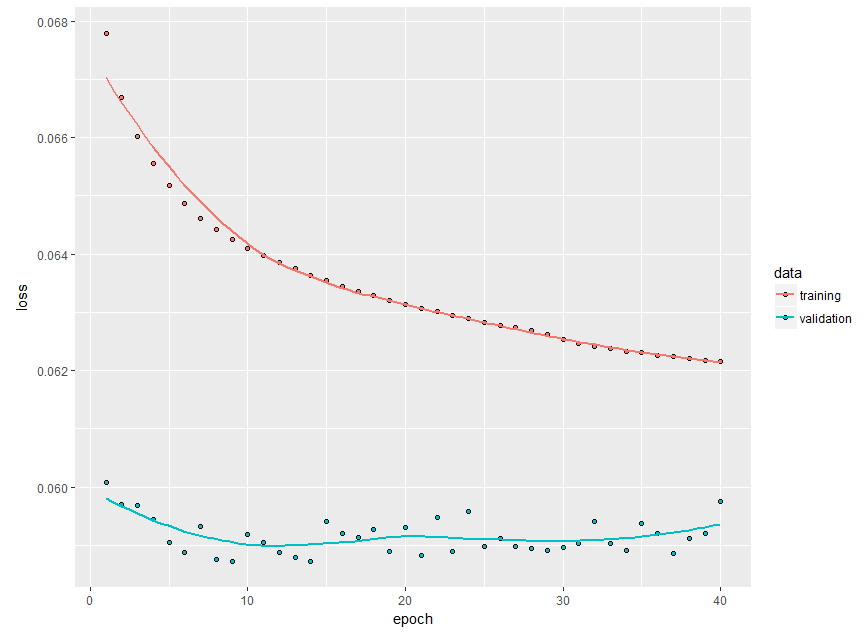
\includegraphics[width=\textwidth]{figures/non_seasonal_residual_history.png}
	\caption{Training and validation loci during the fitting of the non-seasonal RNN model. Note that since we trained the RNN on the residuals of the ETS model, the values for the loss here are not in the same scale as the model's forecasts.}
	\label{fig:non_seasonal_residual_history}
\end{figure}

\subsubsection{Comparison to baseline measure}
As mentioned in section \ref{sec:baseline_methods_non_seasonal}, the baseline statistical forecasting method chosen for the non-seasonal data was the random-walk with drift model (RW model). Using the MAE as the error measure, the RW model outperformed our hybrid model. The MAE of the hybrid model on the test set was 1183.167. The MAE of the RW model on the test set was 1017.714.

\begin{figure}[ht]
	\centering
	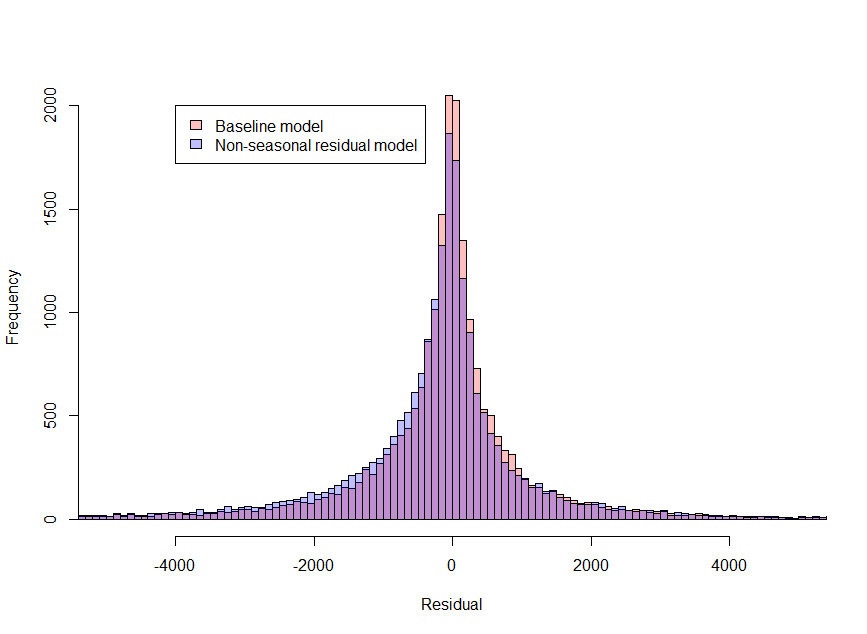
\includegraphics[width=\textwidth]{figures/non_seasonal_res_vs_baseline.png}
	\caption{Distributions of the residuals of the non-seasonal hybrid model and the baseline RW model shown as overlapping histograms. Both sets of residuals are normally distributed, but the variance of the hybrid model's residuals is higher.}
	\label{fig:non_seasonal_res_vs_baseline}
\end{figure}

The distributions of the residuals for both models are shown in figure \ref{fig:non_seasonal_res_vs_baseline}. Both sets of residuals are normally distributed, but the standard deviation of the RW model's residuals is 2273.058, and the standard deviation of the hybrid model's residuals is 2643.934.

\subsubsection{Comparison to ETS model}
Since the ETS model described in section \ref{sec:non_seasonal_stats_modelling} is used to scale the input to the RNN in our hybrid model, it makes sense to compare the performance of our model with that simpler ETS model. The ETS model outperformed our hybrid model just slightly. The MAE of the non-seasonal ETS model on the test set was 1159.775.

\begin{figure}[ht]
	\centering
	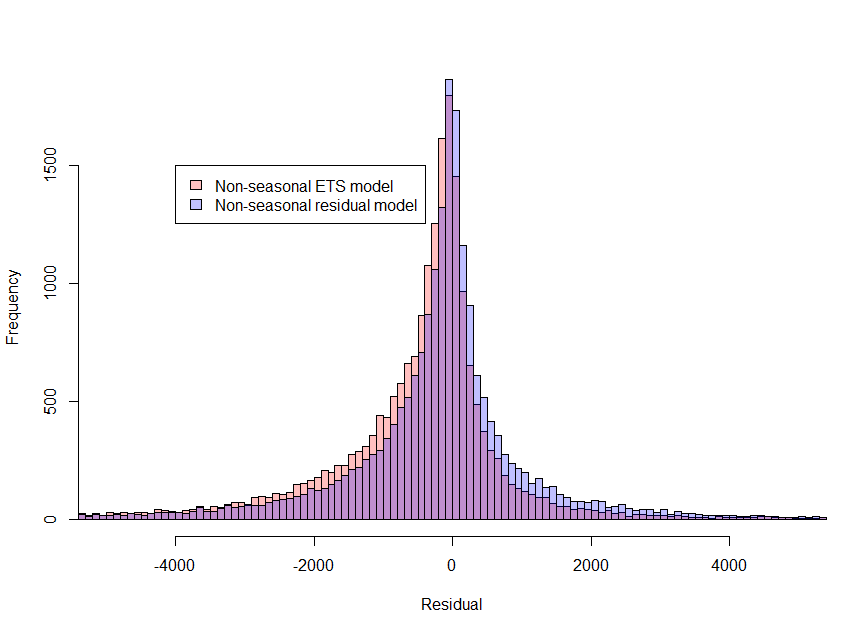
\includegraphics[width=\textwidth]{figures/non_seasonal_res_vs_non_seasonal_ets.png}
	\caption{Distributions of the residuals of the non-seasonal hybrid model and the non-seasonal ETS model shown as overlapping histograms. Both sets of residuals are normally distributed, but the variance of the hybrid model's residuals is higher.}
	\label{fig:non_seasonal_res_vs_non_seasonal_ets}
\end{figure}

The distributions of the residuals for both models are shown in figure \ref{fig:non_seasonal_res_vs_non_seasonal_ets}. Both sets of residuals are normally distributed, but the standard deviation of the ETS model's residuals is 2356.307, and the standard deviation of the hybrid model's residuals is 2643.934.

\subsubsection{Comparison to Meta-learning model}


\subsection{Seasonal Model}
\subsubsection{RNN Training}
There were  \num[group-separator={,}]{24000} quarterly time series in the M4 dataset. We divided these series into a training set of  \num[group-separator={,}]{17000} series, a validation set of  \num[group-separator={,}]{3500}, and a test set of  \num[group-separator={,}]{3500} series. Similar to \ref{sec:non_seasonal_rnn_training}, we fit the model using the training and validation set. We used the mean absolute error as the loss function. See figure \ref{fig:non_seasonal_residual_history} for the training and validation progression during training. Fitting took about $19$ hours. Since the validation loss is increasing while the training loss decreases, the model appears to be overfiitting throughout training. 

\begin{figure}[ht]
	\centering
	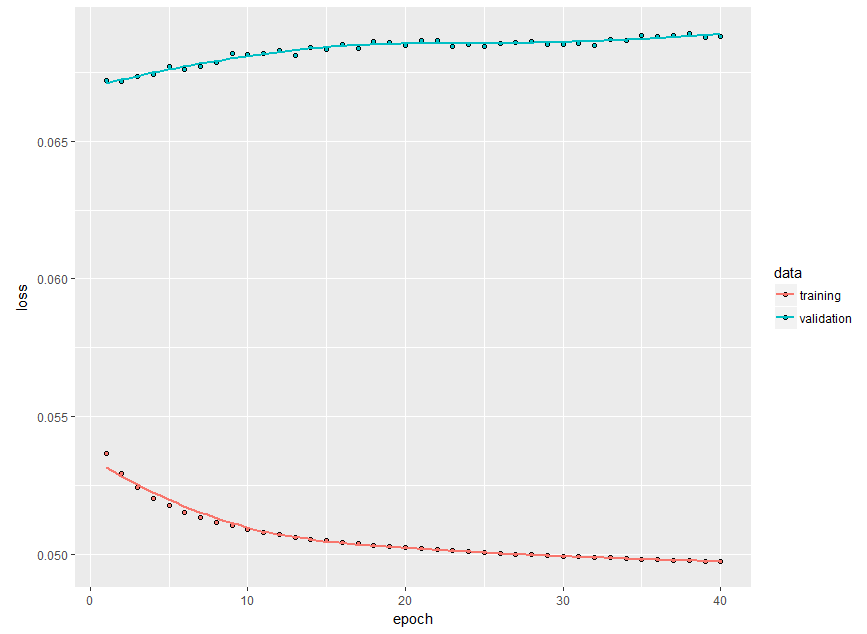
\includegraphics[width=\textwidth]{figures/seasonal_residual_history.png}
	\caption{Training and validation loci during the fitting of the seasonal RNN model. Note that since we trained the RNN on the residuals of the ets model, the values for the loss here are not in the same scale as the model's forecasts.}
	\label{fig:seasonal_residual_history}
\end{figure}

\subsubsection{Comparison to baseline measure}
As mentioned in section \ref{sec:baseline_methods_seasonal} the baseline statistical model for seasonal data was the seasonal na{\"i}ve model. Using the MAE, our hybrid model outperformed the baseline model. The MAE of the hybrid model on the test set was $718.4464$. The MAE of the seasonal na{\"i}ve model on the test set was $854.3212$. 

\begin{figure}[ht]
	\centering
	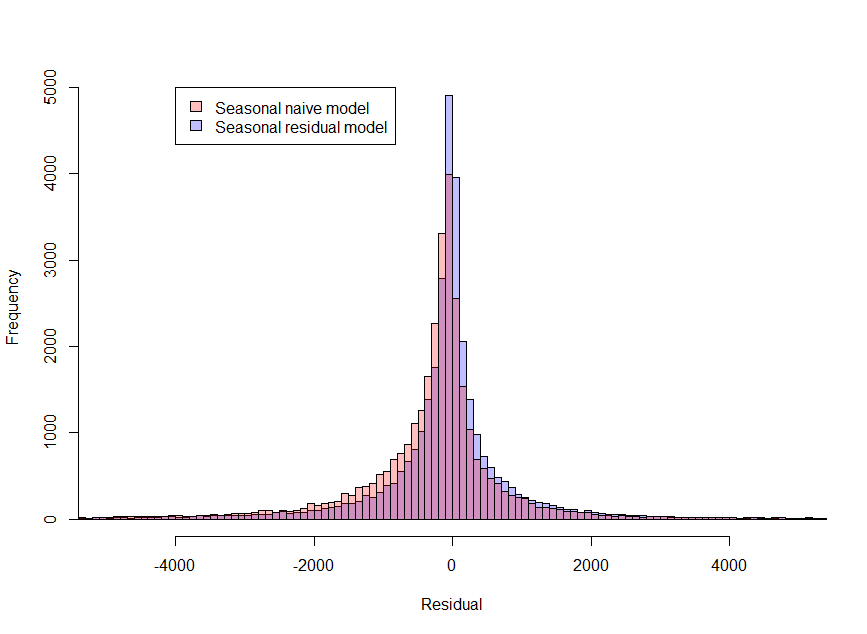
\includegraphics[width=\textwidth]{figures/seasonal_res_vs_seasonal_naive.png}
	\caption{Distributions of the residuals of seasonal hybrid model and the baseline seasonal na{\"i}ve model shown as overlapping histograms. Both sets of residuals are normally distributed, but the variance of the seasonal na{\"i}ve model's residuals is higher.}
	\label{fig:seasonal_res_vs_seasonal_naive}
\end{figure}

The distributions of the residuals for both models are shown in figure \ref{fig:seasonal_res_vs_seasonal_naive}. Both sets of residuals are normally distributed, but the standard deviation of the seasonal na{\"i}ve model's residuals is 1781.011, and the standard deviation of the hybrid model's residuals is 1621.367.

\subsubsection{Comparison to ETS model}
The ETS model described in section \ref{sec:seasonal_stats_modelling} is used to the scale the seasonal data before using it as input for the RNN. So it makes sense to compare our hybrid model to the performance of that ETS model. The ETS model and our hybrid model had almost exactly the same MAE. The MAE of the ETS model was $718.6298$.

\begin{figure}[ht]
	\centering
	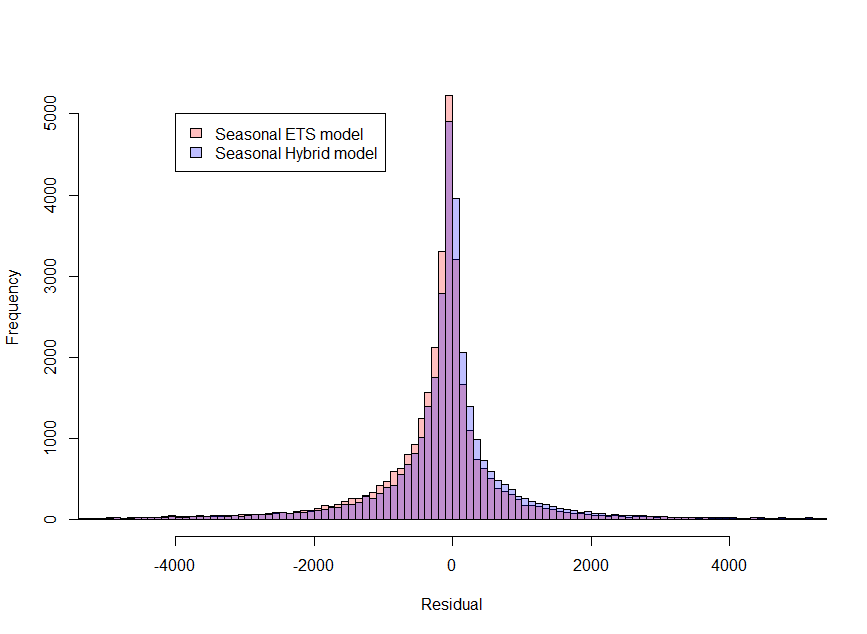
\includegraphics[width=\textwidth]{figures/seasonal_res_vs_seasonal_ets.png}
	\caption{Distributions of the residuals of the seasonal hybrid model and the seasonal ETS model shown as overlapping histograms. The distributions are very similar.}
	\label{fig:seasonal_res_vs_seasonal_ets}
\end{figure}

The distributions of both models are shown in figure \ref{fig:seasonal_res_vs_seasonal_ets}.

\begin{table}\label{tab:performance_summary}
  \centering
  \begin{tabular}{| l | l | c |}
    \hline
    \textbf{Dataset} & \textbf{Model} & \textbf{Mean Absolute Error} \\ \hline
    Yearly & Random Walk with Drift & 1017.714 \\ \hline
    Yearly & Non-seasonal ETS & 1159.775 \\ \hline
    Yearly & Non-seasonal Hybrid & 1183.167 \\ \hline    
    Quarterly & Seasonal Hybrid & 718.446 \\ \hline
    Quarterly & Seasonal ETS & 718.6298 \\ \hline
    Quarterly & Seasonal Na{\"i}ve & 854.3212 \\ \hline
  \end{tabular}
  \caption{A breakdown of the performances of the models applied to their respective datasets.}
  \label{tab:performance_summary}
\end{table}

\section{Conclusions}
\subsection{More Complexity Required}
The hybrid model developed in Uber is much more complicated than the hybrid model described in this document. For example, 
\begin{itemize}
  \item Uber's networks us LSTM units as opposed to GRU units.
  \item Uber's networks have more layers.
  \item The connections between the layers, and the time steps in Uber's networks are more complicated. Uber's networks make use of dilation and attention mechanisms.
  \item The process of scaling using the level and seasonal components is a part of Uber's learning process, as opposed to a pre-processing step, as it is here.
\end{itemize}
Given that our hybrid model was unable to outperform simple statistical methods, it is safe to conclude that additional complexity, like the complexity we see in Uber's model, is required for a more successful forecasting method.

\subsection{Further Research}
There is months of potential further work to be done. We could experiment with the training of the networks by perturbing the number of epochs, introducing early stopping, using different loss functions, using different optimisers etc. 

We could experiment with the network itself by using LTSM units or JANET units in place of GRUs. We could add more layers. We could add attention mechanisms, or dilation mechanisms. We could add residual connections. We could add convolutional layers at shallower layers above the RNN. 

Finally, we only trained and tested on the M4 dataset. The origins of these time series are somewhat foggy. Only the time points, values, and a `type' classifier are given for each time series. It would be worthwhile using time series from more transparent alternative sources.

\newpage

\bibliography{rnn_implementations.bbl}

\end{document}